\chapter{Introdução}\label{cap:intro}

% O Capítulo \ref{cap:intro} é dedicado a uma introdução ao tema do trabalho, descrevendo as ideias gerais do problema em foco e a sua importância. Devem ainda ser explicitados os objetivos do trabalho, clarificada a estrutura do relatório e indicadas as convenções tipográficas.

\section{Enquadramento}

% Deve haver um enquadramento introdutório, que descreva o contexto em que o trabalho se insere, referenciando a proposta original do projeto, que deve constar no primeiro apêndice do documento (ver apêndice \ref{apendice1}).

%TODO artigo que mostra o impacto da tecnologia na industria, forçando a evolução do ambiente industrial
%TODO artigo que mostra a diferença entre empresas que monitoram processos e empresas que nao fazem esse monitoramento 
No cenário industrial contemporâneo, a busca constante por eficiência e inovação tornou-se um pilar essencial para a competitividade e sustentabilidade financeira das empresas. À medida que a tecnologia avança, a produção industrial sofre uma evolução para se manter competitiva perante ao mercado. Nesse contexto, o monitoramento e a otimização das máquinas em linhas de produção tornam-se cruciais para garantir um funcionamento eficaz e prevenir potenciais paralisações ou falhas operacionais.

%TODO artigo que mostra sobre a quantidade de empresas que ainda usam pouca tecnologia no ambiente produtivo
%TODO artigo que mostra perdas na industria por tecnologia desatualizada
No entanto, a tradição das práticas industriais muitas vezes é caracterizada por inspeções manuais e sistemas de monitoramento desatualizados, que não conseguem fornecer informações em tempo real ou análises aprofundadas sobre o desempenho das máquinas. Esse descompasso tecnológico pode resultar em perdas significativas, em termos de produção, de recursos financeiros e manutenção de máquinas.

%TODO Buscar artigo que mostra a diferença entre a quantidade de dados gerados e a quantidade de dados utilizados, mostrando a discrepância e que poucos dados sao realmente utilizados
Além disso, com a crescente integração de sistemas de IoT e a proliferação de sensores avançados, existe uma quantidade imensa de dados sendo gerada continuamente. No entanto, sem a infraestrutura adequada para coletar, armazenar e analisar esses dados, as empresas podem se encontrar sobrecarregadas, incapazes de extrair insights significativos que poderiam informar decisões estratégicas e operacionais.

Com esse contexto de mercado, uma empresa da industria de estampagem buscou a construção de projetos que realizem a sensorização de suas maquinas, armazenamento e tratamento dos dados, e a visualização dessas informações, de forma a se tornar mais competitiva, eficiente e lucrativa. Esses projetos foram agrupados dentro do contexto “ATTRACT - Digital Innovation Hub for Artificial Intelligence and High-Performance Computing - Project: 101083770 — ATTRACT — DIGITAL-2021-EDIH-01”, com financiamento “Digital Europe Programme (DIGITAL) - DIGITAL-2021-EDIH-INITIAL-01 — Initial Network of European Digital Innovation Hubs”, chamado de \texttt{Projeto Attract} nesse documento.

\section{Objetivos}

% Os objetivos do trabalho devem ser apresentados de forma clara e compatível com a proposta original do projeto. Na eventualidade de os objetivos originais terem sido reformulados, devem ser apresentadas as razões objetivas que conduziram a essa reformulação.

% Idealmente, deve-se incluir um cronograma do projeto, indicando explicitamente as tarefas realizadas e o tempo dedicado a cada uma. Existindo um cronograma na proposta original do projeto, deverão justificar-se eventuais discrepâncias com o cronograma real.


%TODO artigo sobre a quantidade massiva de dados que é produzida em excesso
Dado o enquadramento anterior, a necessidade identificada é de desenvolver um sistema robusto que possa receber dados de sensores que coletam dados das máquinas em tempo real, armazená-los de maneira eficiente em um data lake e apresentá-los através de um dashboard, transformando a maneira como a empresa monitora e otimiza sua linha de produção, garantindo não apenas eficiência, mas também uma abordagem proativa à manutenção e gestão industrial. Esse sistema não apenas forneceria informações em tempo real sobre o status e o desempenho das máquinas, mas também permitiria análises históricas, ajudando gestores e técnicos a identificar tendências e falhas, além de otimizar a produção, minimizando perdas na produção e otimizando os ganhos financeiros.

\section{Estrutura do Documento}
%TODO referencia para o crescimento da demanda por analise de dados
Esta dissertação de mestrado está organizada começando pela Introdução, onde o problema e o escopo são apresentados. Esta seção contextualiza a necessidade de modernização industrial, destacando a importância do monitoramento e otimização de máquinas na indústria. A relevância do estudo é então justificada, com foco na crescente demanda por análise de dados no mercado.

Segue-se com a Revisão Literária, que apresenta uma análise sobre trabalhos e conceitos relacionados ao projeto. Esta seção engloba trabalhos semelhantes já realizados nas partes de recebimento de dados em tempo real, processamento e alertas.

A Metodologia discute a escolha de tecnologias específicas usadas no projeto, detalhando o método de armazenamento de dados, e o processo adotado para o desenvolvimento do software, e também são descritas as estratégias de gestão das atividades do projeto.

No capítulo sobre a Arquitetura do Sistema, é discutido sobre as especificidades técnicas do sistema proposto. Desde o diagrama geral do sistema até a forma como cada parte do sistema está organizada, deixando claro como cada parte é organizada e como ocorre a interação entre elas.

No capítulo de Implementação, aprofunda-se nos aspectos técnicos do sistema. Aqui, cada componente do banco de dados, da \gls{API}, do módulo de processamento de dados, do modulo de recebimento de dados e do frontend, são detalhadamente descritos. Esse capítulo visa mostrar de forma prática como foi implementada a arquitetura detalhada no capítulo anterior.

No que diz respeito às Características do Sistema do ponto de vista funcional, a dissertação tem uma seção que foca em mostrar a aplicação prática do software, mostrando como cada funcionalidade funciona e como ocorrem as interações com o usuário.

Em Resultados e Avaliação, são apresentados os resultados obtidos durante o projeto, destacando as principais realizações e benefícios observados na implementação do sistema proposto. A Conclusão e Trabalhos Futuros resume os pontos chave do projeto, identifica as limitações do sistema atual e sugere possíveis direções para continuidade e implementações futuras.


% \section{Normas de Composição}

% Para além de uma organização que reflita o percurso seguido, o relatório deve estar bem formatado e ter aspeto sóbrio, convidando à leitura e fazendo jus ao mérito do trabalho descrito. Neste sentido, apresentam-se de seguida algumas das normas a levar em conta\footnote{Estas normas, assim como este modelo de documento, são compatíveis com o preconizado no "Regulamento da Unidade Curricular de Projecto das Licenciaturas", designadamente no que diz respeito ao relatório do projeto.}.

% \subsubsection{Convenções Tipográficas}

% Por vezes, opta-se por apresentar as convenções tipográficas seguidas no documento, ou seja, em que circunstâncias se usam texto em \textit{itálico}, \textbf{negrito}, ou de \texttt{espaçamento uniforme} (esta última formatação é normalmente usada para apresentar código fonte), bem como quais as fontes tipográficas usadas, respetivas dimensões, etc.


% \subsubsection{Tabelas e Figuras}

% Tabelas e figuras devem ser numeradas automaticamente e ter um tamanho equilibrado (nem muito grande, nem muito pequeno), como a Tabela \ref{tab:exemplo_de_tabela} e as Figuras  \ref{fig:exemplo_de_figura}, \ref{fig:exemplo_de_figura2} e \ref{fig:exemplo_de_figura3}.

% \begin{table}[htbp]	
% 	\centering
% 	{\small
% 		\begin{tabulary}{\linewidth}{|L|C|R|}	
% 			\hline 	
% 			{\bf Nome da Coluna 1} & {\bf Nome da Coluna 2} & {\bf Nome da Coluna 3} \\ 
% 			\hline 
% 			conteúdo A & conteúdo B & conteúdo C \\ 
% 			\hline 
% 			conteúdo D & conteúdo E & conteúdo F \\ 
% 			\hline 
% 		\end{tabulary} 
% 	}	
% 	\caption{\small{Exemplo de tabela.}}
% 	\label{tab:exemplo_de_tabela}
% \end{table}


% \begin{figure}[htbp]
% 	\centering
% 	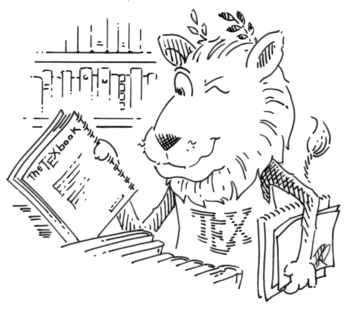
\includegraphics[scale=0.75]{images/lion_large}
% 	\caption{Exemplo de imagem PNG.}
% 	\label{fig:exemplo_de_figura}
% \end{figure}

% Sempre que possível, devem-se usar formatos escaláveis (e.g., PDF), como na Figura \ref{fig:exemplo_de_figura2}, e evitar imagens comprimidas (formatos JPG, PNG, GIF, etc.), como na Figura \ref{fig:exemplo_de_figura}.

% \begin{figure}[htbp]
% 	\centering
% 	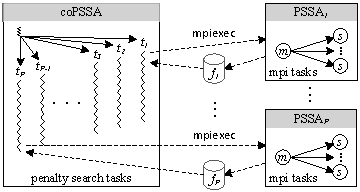
\includegraphics[width=0.75\linewidth]{images/architecture}
% 	\caption{Exemplo de imagem PDF.}
% 	\label{fig:exemplo_de_figura2}
% \end{figure}


% Em gráficos devem-se indicar sempre as grandezas associadas a cada eixo, bem como a respetiva legenda -- ver exemplo na Figura \ref{fig:exemplo_de_figura3}. Adicionalmente, o esquema de cores ou de traços para as linhas, deve ser sóbrio e prevenir ambiguidades na leitura do gráfico.

% \begin{figure}[htbp]
% 	\centering
% 	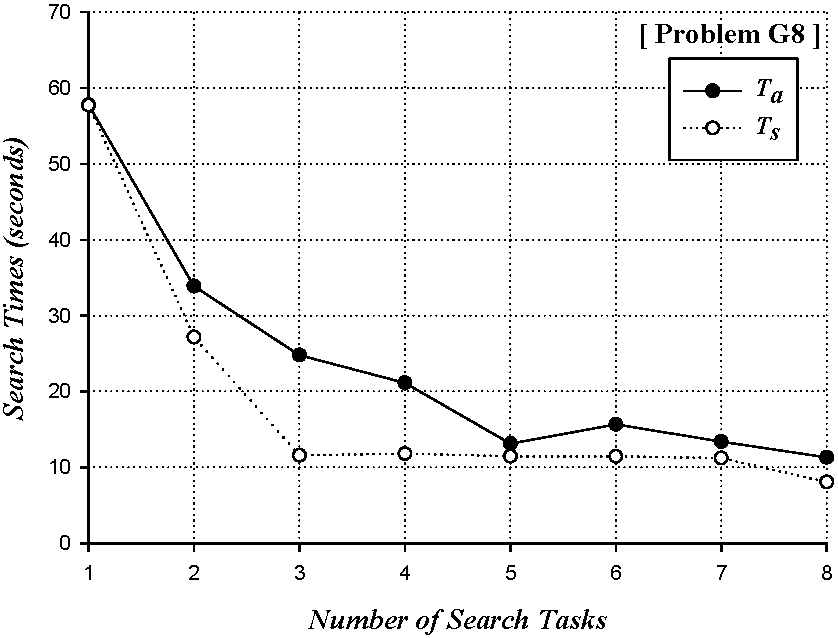
\includegraphics[width=0.65\linewidth]{images/search_times}
% 	\caption{Exemplo de gráfico.}
% 	\label{fig:exemplo_de_figura3}
% \end{figure}

% \subsubsection{Distribuição dos Elementos}
% A forma como o texto e outros elementos (tabelas, figuras, etc.) se distribui por uma página, deve ser tal que se evitem grandes blocos vazios no final da página. Embora algumas sistemas de composição tendam a garantir isso automaticamente (como o LaTeX), é costume serem necessárias afinações para resolver, manualmente, essas (e outras) desformatações. No entanto, essas afinações devem ser deixadas para a fase pré-impressão, já com o conteúdo do documento estabilizado, de forma a evitar trabalho inconsequente.


% \subsubsection{Correcção Ortográfica}
% Para além da qualidade tipográfica do relatório, é imprescindível minimizar (se possível até, erradicar) erros ortográficos. Qualquer sistema de composição de documentos suporta correção ortográfica (e, muitas vezes, sintática), pelo que não é aceitável a submissão para avaliação de relatórios sem revisão ortográfica prévia.


% \subsubsection{Referências Bibliográficas}
% Ao longo do documento, deve ficar sempre perfeitamente claro o que é escrita original e o que foi baseado (ou até reproduzido de) noutras fontes. 

% Todas as fontes devem ser descritas na formatação usada na Bibliografia e referenciadas, no texto, pelos seus identificadores únicos. Por exemplo: ``Uma solução para o problema em causa deve respeitar as propriedades {\it x}, {\it y} e {\it z} \cite{INPROC1}.'', ou ``Neste trabalho explorou-se a API PThreads \cite{TECH01} com o objetivo de $\dots$''.  No modelo em LaTeX, as referências bibliográficas são definidas no ficheiro {\tt libs/refs.bib}, onde existem entradas de diferentes tipos: livro \cite{BOOK01}, artigo de conferência \cite{INPROC1}, relatório técnico \cite{TECH01} e sítio web \cite{FORD11}.

% A reprodução fiel de texto de fontes externas deve ser limitada, surgir entre aspas, ligeiramente destacada, e ter apensa a respetiva referência bibliográfica.  Por exemplo:

% \begin{quotation}
% ``Recently, the employment of GPU devices is a key to achieve higher performance for computer systems. On those systems, GPUs are used for general calculation but with extreme parallelism.'' \cite{INPROC1}
% \end{quotation}

% \subsubsection{Siglas}
% Na primeira vez as siglas devem surgir por extenso, sendo resumidas nas vezes seguintes. Por exemplo: ``o curso atual de Engenharia Informática da \gls{ESTiG} foi reformulado em 2015 e, a par com o curso de Informática de Gestão, representa o leque de licenciaturas da área de Informática que a \gls{ESTiG} oferece''. No modelo em LaTeX, as siglas são definidas no ficheiro {\tt acronym.tex}.



